%************************************************
\chapter{Problem Statement}\label{ch:problemstatement}
%************************************************

This section will further define the problem and derive formal requirements to event subscription mechanisms

illustrate the complexity through 2 sample scenarios that are similar but different

\section{Motivating Examples}
% some has been mentioned in the introduction

To allow a better understanding of the issue, event-driven use-cases from two different domains are presented in the following.
The cases are revealed through their standard BPMN representation, which can cause problems in certain real-life situations.
It is illustrated, why the time of event subscription is of great importance and motivate to study the mechanics and implications of event subscription in business processes.

\paragraph{Delay of a logistics process}
The first example(\autoref{fig:example-eurotunnel}) is taken from the logistics domain and shows a truck transport that has to cross the English Channel.
The truck driver receives the transport plan for his next tour from France to the UK. By default, the company crosses the Channel using the Eurotunnel, an underground train connection between London and Paris.

\begin{figure}[]
	\myfloatalign
	{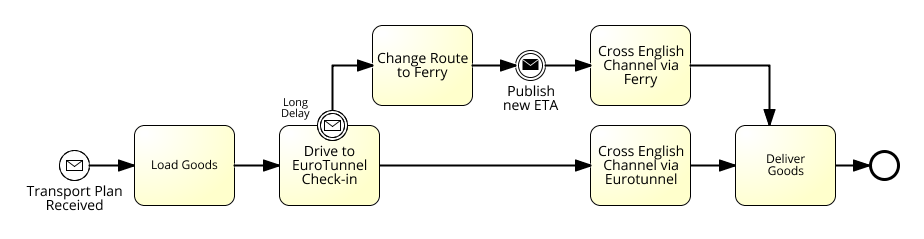
\includegraphics[width=1\linewidth]{chapters/requirements/Eurotunnel-simplified.png}}
	\caption{BPMN Model of a Logistics Process using events for route optimization (Example 1.1)}
	\label{fig:example-eurotunnel}
\end{figure}

After loading the goods at the factory, the truck will head towards the check-in location of the Eurotunnel.
If everything runs on schedule, the truck will cross the channel on the train and then deliver the goods in Great Britain.
Alternatively, the process considers a route using the ferry from Calais(FR) to Dover(UK).
The Eurotunnel administration publishes delay information approximately every 30 minutes through an RSS feed on their website. While it mostly operates on schedule, delays ranging from 15~minutes to several hours occur regularly. It can happen that new information is not published for multiple hours.
Significant delay events (delay~>~30~minutes) are received through a boundary catching message event attached to the activity \textit{Drive to Eurotunnel Check-In}. The boundary event is interrupting, hence the activity is canceled if a delay occurs.
The transport continues towards the ferry terminal and crosses the English Channel over sea. After crossing the channel, the goods are delivered to the recipient.
\todo[inline]{show a cep query for that scenario to make it more precise}

According to the BPMN specification, the listening for the boundary event starts as soon as the related activity is activated.
\todo[inline]{is that exactly correct?}
Given that events arrive every 30~minutes, there can be a gap of up to half an hour, before the first information becomes available.
In the worst cases, when data isn't published for several hours, this gap will be even bigger.
Let's consider a very busy weekday. A technical fault occurred in the tunnel earlier and the train runs 3 hours behind schedule.
The last information on the RSS feed was published at 2:35pm. At that time the truck driver is still in the process of loading goods, finishing the activity at 2:40pm.
Following the process definition, the driver now departs towards the Eurotunnel check-in.
The system publishes updated information at 3:15pm: operations are still 2:30h behind schedule. The message gets received through the process and the truck driver takes the alternative route to the ferry, but only after heading to the Eurotunnel for 35~minutes. The late change of plans causes an unnecessary delay to the shipment.

\begin{figure}[]
	\myfloatalign
	{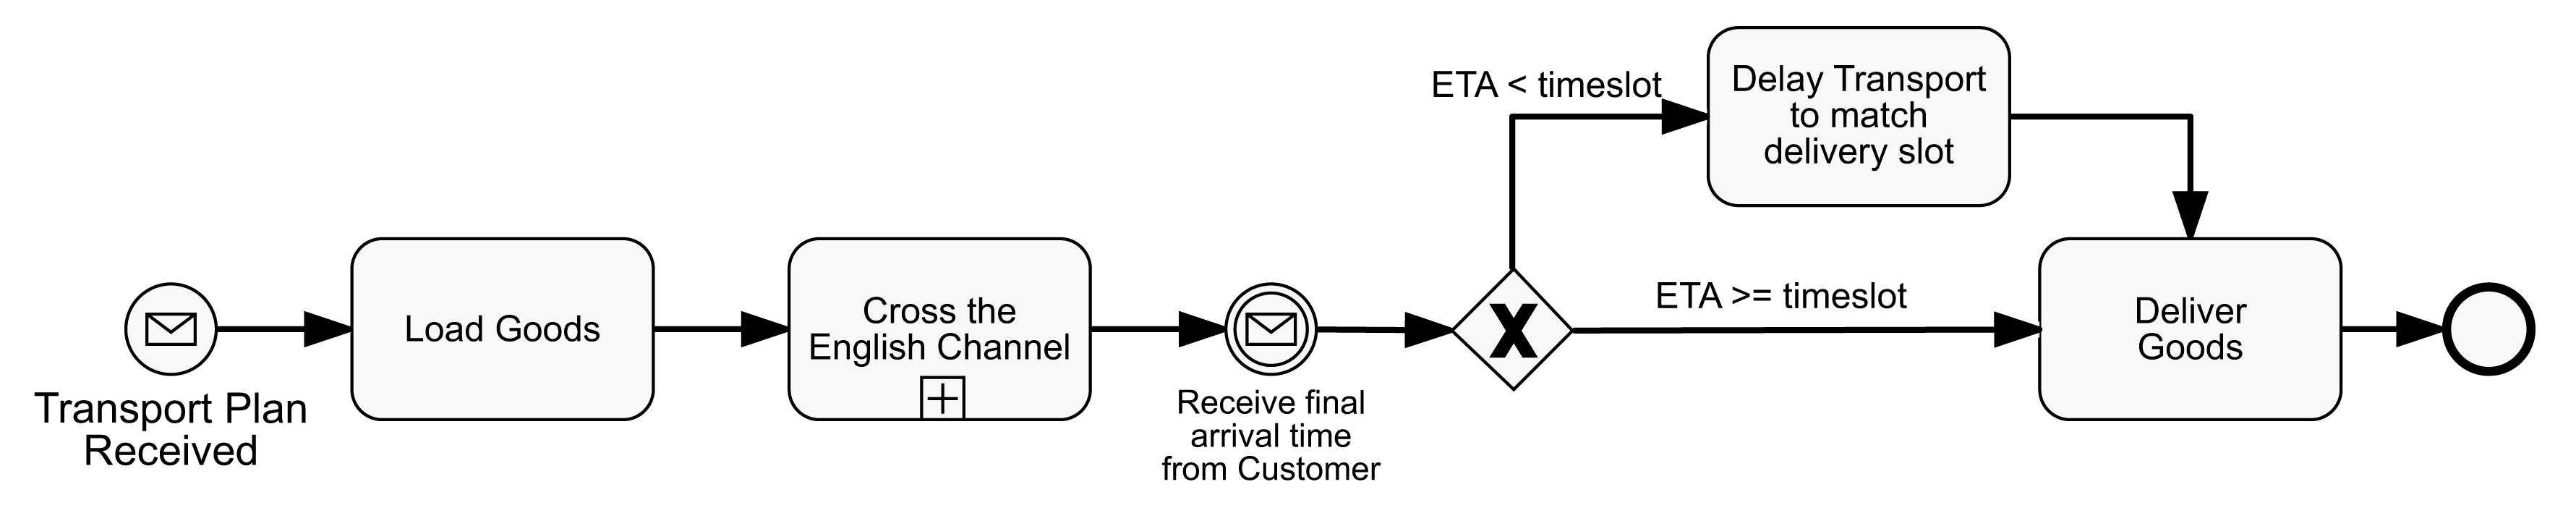
\includegraphics[width=1\linewidth]{chapters/requirements/Eurotunnel_part2.png}}
	\caption{Transport via English Channel that is timed to a delivery slot (Example 1.2)}
	\label{fig:example-eurotunnel-part2}
\end{figure}

\autoref{fig:example-eurotunnel-part2} is an extension of the the transport process.
In logistics, it is common that a delivery cannot be accepted at arbitrary time. Instead, the receiving party assigns delivery windows to the transport company.
The transport must arrive during the given time window, otherwise the delivery cannot be completed.
After crossing the English Channel, the process model shows the catching of a message event containing the desired final arrival time at the factory. There is an agreement with the factory, that the delivery slots will be approved 2~hours before the expected arrival.
If the current ETA of the transport is greater or equal to the arrival time, the driver will head to the drop-off point straight away. If the transport is ahead of schedule, the driver will have to delay the delivery to match the time window.

The presented process model illustrates another complexity of using events in processes. Again, the listening to the announcement of a delivery window will start when the event element is reached, in this case only after crossing the English Channel. 
Until an event has been received, the process will not continue. 
Much worse: if the receiving party sends out the arrival time information too early, while the truck is crossing the channel, the event is missed. If it is not issued again, the process cannot receive a message and will get stuck indefinitely waiting to catch the event.

Neither of the two presented catch events allow for an efficient and reliable execution of the process. They can cause unnecessary delays and even blocking of the process execution.
The remainder of this work will further analyze the capabilities of BPMN to express event-usage scenarios and propose solutions to the mentioned problems.

\todo[inline]{Consider more possible event occurrence times to prepare for the next chapter}

\paragraph{Up-to-date shipping information for an order}
\begin{figure}[]
	\myfloatalign
	{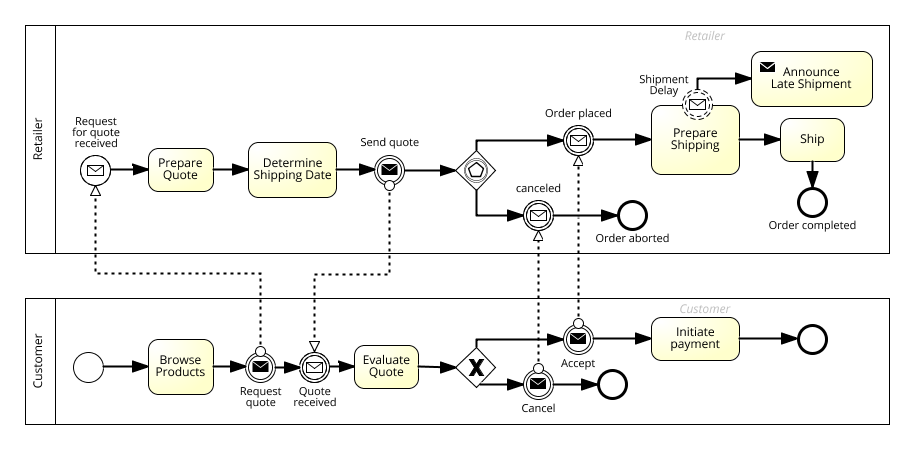
\includegraphics[width=1\linewidth]{chapters/requirements/Retail-Order.png}}
	\caption{Model of a retail order management process (Example 2)}
	\label{fig:example-order}
\end{figure}

A~similar situation can be observed in the Order Management process presented in \autoref{fig:example-order}.
It describes the interaction between customer and seller in a traditional distance retail scenario: After browsing the product catalog, the customer requests a quote for the articles he or she is willing to buy.
The retailer makes an offer including an approximation of the expected shipment date and sends it to the customer. That quote is then either accepted or not and the payment is issued if necessary.
Once the retailer is informed about the placement of the order, the products are packed and shipped as soon as possible.
For articles that are not currently in stock, the retailer must await the shipment from the factory. If any of the factory-shipments is delayed, the retailer cannot ship in time and will announce a delayed shipment date to the customer.
This situation is modeled through a non-interrupting boundary event attached to the \textit{Prepare Shipping} activity, which triggers the sending of the updated shipment date to the customer.

The process shows a number of similarities, but also differences in terms of event-use when compared to the previous process example.
At first we want to look at the three intermediate catch events, \textit{Quote received}, \textit{Order canceled} and \textit{Order placed}.
In each of the cases, the event to be caught is the direct response to a message that was sent right before. While the process will also enter a waiting state until the response arrives, that waiting is not to be interpreted as an unnecessary delay to the process execution.
Other than in Example~1.2(\autoref{fig:example-eurotunnel-part2}), there is nothing useful to do before the response is received.
It is furthermore worth noting that the response messages cannot be missed, because the message catch event immediately follows the message send event.

A different situation holds for the boundary event \textit{Shipment Delay}.
While the subscription to a Eurotunnel event can be issued at any time, it does not depend on any process data, the shipment delay has to be observed for each product that is part of the order. A subscription can therefor not be executed before the activity \textit{Prepare Quote} has finished executing  \todo[inline]{show a cep query for that scenario to make it more precise}
By process definition, the system will listen to shipment delays once the activity \textit{Prepare Shipping} has started executing, much later than possible.
Any events that occur between the two activities, that means, for example, when the customer makes the decision about accepting or canceling the order, cannot be considered in the process execution and the customer will not be informed about a possible late shipment.


% The first of these three follows the \textit{Send/Receive} Service Interaction Pattern. \todo[inline]{missingref}
% Two parties interact 
\todo[inline]{write about service interaction patterns somewhere}

\paragraph{}
\noindent
The two presented examples have illustrated the complexity of using events in business process, especially when the possible event occurrence times are considered in detail.
Differences have been pointed out as to how exactly the event is placed in the process, if it waits for a direct response to an earlier request or if the event occurrence unrelated to the execution of that very process.
Motivated by this complexity, it is the goal of this work to identify the capabilities of BPMN to handle event subscription in business processes.

\todo[inline]{this chapter must be closer related to event subscription. Don't make it too general. subscription is the thing}


\section{Event Occurrence Scenarios}
Given the motivating examples, I am deriving a generic set of event occurrence scenarios. Each of these scenarios can occur in the real world and process implementations need to be capable of handling them to avoid negative effects.

\paragraph{Event Subscription Time}

The most important variable to consider is the time of event occurrence. \todo[inline]{reformulate}
According to the BPMN specification, it is possible to catch an event if it occurs after the event element is enabled. As shown before, it is often impossible to control occurrence time and events do occur outside of these time windows.
We specify the possible event occurrence times in relation to the life cycle of a process that utilizes a BPMN Intermediate Event \todo[inline]{ref process lifecycle}.
\begin{figure}[]
	\myfloatalign
	{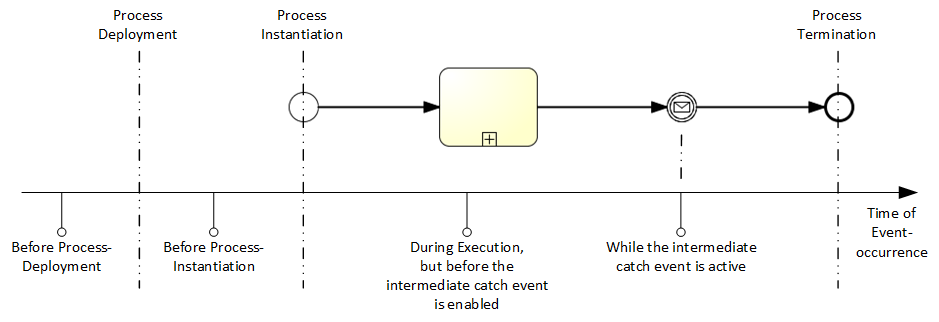
\includegraphics[width=1\linewidth]{chapters/requirements/timeline-event-occurrence.png}}
	\caption{Possible event occurrence times in relation to a process execution life cycle}\label{fig:occurrence-timeline}
\end{figure}

\autoref{fig:occurrence-timeline} shows the life cycle steps of a process and an instance from the deployment of the process until the undeployment and uses a timeline to illustrate that an event might occur at any time during this cycle. More precisely, an event is always considered to occur before or after a life cycle step or in between two consecutive steps.
\todo[inline]{How about system-deployment/process engine start and process undeployment? show in illustration, but say in text that we simplify this for now. after undeployment is essentially before deployment of a new process; Before Engine start is also before pr. deployment and we presume that an engine is running and does not stop.}

Given the relevant life cycle steps, \textit{process deployment}, \textit{process instantiation} and \textit{Event enablement}, the following occurrence scenarios are distinguished in this work:
\begin{aenumerate}
	\item O1 After the enabling of the BPMN event (BPMN default)
	\item O2 The event does not occur
	\item O3 Between Process instantiation and the enabling of the BPMN event
	\item O4 Between Process deployment and process instantiation
	\item O5 Before Process deployment
\end{aenumerate}\label{def:occurrence-times}

\todo[inline]{add a back reference to the examples. In example XY, events can occur before... whereas in example...}

For a flexible and efficient use of events in business processes, it must be possible to use events that occur in any of these phases.
To make sure that an event can be caught, no matter at which time during the phase it occurs, the subscription to the CEP platform must happen at the beginning of the occurrence phase.
It follows that the event subscription must be possible at system start, at process deployment, at process instantiation, at any time during process execution and when the BPMN Event element is enabled.

\todo[inline]{Explain that, to catch events at these times, the subscription has to happen before. Therefor we derive event subscription times}

\paragraph{Event Subscription Dependencies}
It is important to note that the subscription to an event source can depend on additional context information or process data. This can be a significant limitation to the possible subscription time.
\todo[inline]{ref to process model} shows a logistics process that uses event data about the GPS position of a certain truck to keep the estimated time of arrival of the transport updated. Whenever it receives an updated GPS position, the ETA is re-calculated; once the \textit{arrival}-event has been received, the process finishes.

\todo[inline]{this example is not good, because we are not interested in a gps event that occurs earlier. Find an example where you would like earlier events, but subscription is not possible}

Before the subscription to that specific truck gps event can happen, the process must determine the \textit{truckId} to use in the event query. Only when the \textit{truckId} is available, the subscription can be executed. This example illustrates how a query filter expression can depend on context data, but it might as well be the event source itself that differs depending on the particular execution.

\todo[inline]{there could be an xor gateway and following two different events and only one of them can get executed}

\todo[inline]{solution would be to listen to all gps, but potentially too much data. Decision must be made cautiously! <= Where should I mention this? maybe later in the concept}

\todo[inline]{formulate a concise Problem Statement}

\section{Requirements Definition}
\todo[inline]{Maybe move to the end of 4. and add non-functional requirements as well?}

The previous sections have exemplified how the execution semantic offered by the BPMN specification limits users in the use of events in business processes. Now these shortcomings are formalized into an additional set of requirements that must be met by a process execution environment to enable event handling in the extended set of event occurrence scenarios.
The formal requirements will later be used to evaluate the capabilities of current Process Management Solutions~(\autoref{ch:assessment}) and to develop a new concept to handling event subscription in business processes~(\autoref{ch:flexibleeventsubscription}).

\paragraph{R1: Flexible Event Subscription Time}

\begin{description}
	\item[R1.1 Explicitness:] 
	For each event that is used in a business process, it must be possible to derive the time of event subscription from the process model. The time of subscription may either be explicitly stated or defined implicitly.
	\item[R1.2 Flexibility:] 
	The time of subscription can be influenced to catch events according to any of the event occurrence scenarios O1, O2, O3, O4. In other words, the process model defines the earliest acceptable time for an event occurrence to be considered in the process execution. The necessary options are \textit{since system start}, \textit{since process deployment}, \textit{since process instantiation}, from an arbitrary but \textit{explicit time during process execution}, or \textit{since enabling of the Event Process Element}.
\end{description}


\todo[inline]{limited by subscription dependencies}
\todo[inline]{change the options back to the times of subscription. Mention that the subscription is necessary before the time of event occurrence, but too early subscription is also a problem.}
\todo[inline]{target only intermediate events. (limitation, although it also makes the most sense.)}

\paragraph{R2: Automatic Subscription Handling}

\begin{description}
	\item[R2.1 Subscription:] 
	The subscription to event sources is handled implicitly by the process execution environment as defined by the process model.
	\item[R2.2 Removal of Subscription:] 
	The removal of a subscription from the system is handled automatically as soon as a subscription becomes unnecessary.
\end{description}


\begin{description}
	\item[R3 Event Buffering:]
	To make all events since the subscription time available during process execution, matching events need to be stored temporarily.
\end{description}

\todo[inline]{buffer policies?}